%!TEX root = ../dokumentation.tex

% Erste Erwähnung eines Akronyms wird als Fußnote angezeigt. Jede weitere wird
% nur verlinkt: \acf{AGPL}. \cite{fsf:2007}

% Verweise auf das Glossar: \gls{Glossareintrag}, \glspl{Glossareintrag}

% Nur erwähnte Literaturverweise werden auch im Literaturverzeichnis gedruckt:
% \cite{baumgartner:2002}, \cite{dreyfus:1980}

% Meine erste Fußnote\footnote{Ich bin eine Fußnote}

% \begin{wrapfigure}{r}{.4\textwidth}
% \centering
% \includegraphics[height=.5\textwidth]{logo.png}
% \vspace{-15pt}
% \caption{Das Logo der Musterfirma\footnotemark}
% \end{wrapfigure}
% %Quelle muss in Fußnote stehen (da sonst aufgrund eines Fehlers nicht kompiliert
% % wird)
% \footnotetext{aus \cite{mustermann:2012}}

\chapter{Aufgabe}
\section{Carolocup, Regeln}
Der Carolocup ist ein jährlich veranstalteter Hochschulwettbewerb der Universität Braunschweig.
Teams aus Studenten entwickeln ein 1:10 Modelauto. 
Dieses Auto soll in der Lage sein autonom durch einen Parkour zu fahren. 
Die Autos sind meist ausgestattet mit Kameras, Sensoren und einem Rechner auf dem verschiedene Algorithmen zur Auswertung der Daten laufen.

\section{Simulation}
Der Kern dieser Arbeit beschäftigt sich mit dem Aufbau einer Simulationsumgebung.
Das Fahrzeug Hat einen Hardware und einen Software Teil. \\
Im unteren Schaubild befindet sich der Hardwareteil auf der linken Seite.
Das sind zum einen die Sensoren und die Kamera und zum anderen die Fahrmechanik.
Zur Fahrmechanik gehört alles was sich im Fahrzeug bewegt, d.h. Motoren, Servos, Räder\dots\\
Auf der rechten Seite des Schaubilds ist die Fahrzeugsteuerung.
Die Hardware liefert ein Kamerabild und Sensordaten an die Fahrzeugsteuerung.
Auf Basis dieser Daten berechnet die Fahrzeugsteuerung einen geeigneten Lenkwinkel und verändert gegebenen Falls die Geschwindigkeit des Fahrzeugs.
Diese zwei Werte werden dann an die Hardware gegeben, und Motor und Servo werden auf die neuen Werte angepasst.
\begin{center}
    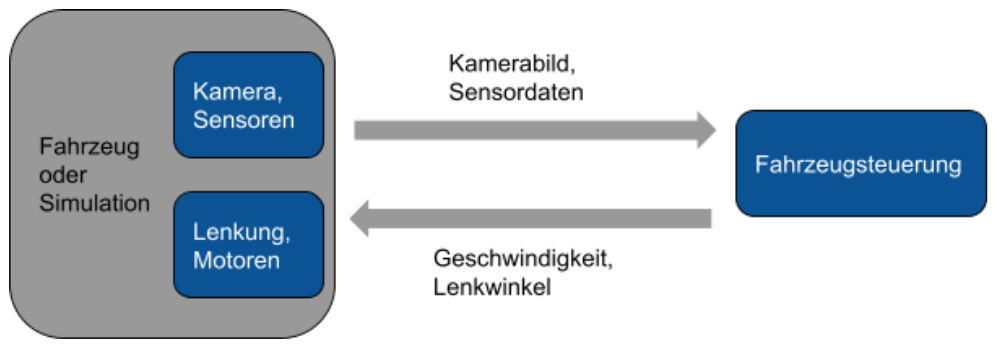
\includegraphics[width=1\textwidth]{SimulationDiagram.png}
\end{center}
Das Ziel einer Simulation ist es den Linken Teil des Schaubilds zu ersetzen.
Statt der Hardware kann man die Fahrzeugsteuerung mit der Simulation laufen lassen.
Die Schnittstelle bleibt die Gleiche: Die Simulation empfängt Lenkwinkel und Geschwindigkeit und errechnet daraus ein Kamerabild und andere Sensordaten.
Dafür müssen sämtliche Hardwarekomponenten virtualiesiert werden. 
Es wird eine 3D-Umgebung benötigt in der sich ein Fahrzeug auf virtuellen Fahrbahnen bewegen kann.
Dadurch kann eine virtuelle Kamera ein Bild erstellen.
Außerdem wird eine Logik benötigt führ die Fahrmechanik. 
Ein Lenkwinkel und eine Geschwindigkeit müssen umgerichnet werden in eine Transformation des Fahrzeugs in der 3D-Umgebung.
\\
\subsection*{Warum Simulation?}
Wenn man den linken Hardware Teil durch eine Simulation ersetzt, ist rechts und links im Schaubild Software.
Man könnte dann an der Fahrzeugsteuerung entwickeln, und neuen Code testen ohne Zugriff auf die Hardware des Fahrzeugs zu haben.
Das ist ein Vorteil wenn viele Leute gleichzeitig am Fahrzeug arbeiten.
Wenn die Simulation Tests auf Knopfdruck bereitstellt, fällt es Entwicklern leichter den Code zu testen.
Dadurch können Feedbackloops, durch öfteres testen bei der Entwicklung, kleiner werden.
Somit werden Bugs oder eine Verschlechterung bestimmten Fahrverhaltens schneller erkannt.

\section{Anforderungen}
Als Basis wird hier die KIT Gazebo Simulation genutzt.
Primäres Ziel der Arbeit ist es eine Schnittstelle zwischen der DHBW Smart Rollerz Fahrzeugsteuerung und der KIT Gazebo Simulation zu schaffen.
Wenn dies gelingt können Funktionen der Simulation, wie die Evaluierung von Fahrten oder die Generation von Strecken genutzt werden.

Neue Sensoren testen wie ToF und Lidar.

